%%%%%%%%%%%%%%%%%%%%%%%%%%%%%%%%%%%%%%%%%%%%%%%%%%%%%%%%%%%%%%%%%%%%%%%
%%                                                                 %%
%% Please do not use \input{...} to include other tex files.       %%
%% Submit your LaTeX manuscript as one .tex document.              %%
%%                                                                 %%
%% All additional figures and files should be attached             %%
%% separately and not embedded in the \TeX\ document itself.       %%
%%                                                                 %%
%%%%%%%%%%%%%%%%%%%%%%%%%%%%%%%%%%%%%%%%%%%%%%%%%%%%%%%%%%%%%%%%%%%%%%%

%%\documentclass[referee,sn-basic]{sn-jnl}% referee option is meant for double line spacing

%%=======================================================%%
%% to print line numbers in the margin use lineno option %%
%%=======================================================%%

%%\documentclass[lineno,sn-basic]{sn-jnl}% Basic Springer Nature Reference Style/Chemistry Reference Style

%%======================================================%%
%% to compile with pdflatex/xelatex use pdflatex option %%
%%======================================================%%

%%\documentclass[pdflatex,sn-basic]{sn-jnl}% Basic Springer Nature Reference Style/Chemistry Reference Style

%%\documentclass[sn-basic]{sn-jnl}% Basic Springer Nature Reference Style/Chemistry Reference Style
\documentclass[sn-mathphys]{sn-jnl}% Math and Physical Sciences Reference Style
%%\documentclass[sn-aps]{sn-jnl}% American Physical Society (APS) Reference Style
%%\documentclass[sn-vancouver]{sn-jnl}% Vancouver Reference Style
%%\documentclass[sn-apa]{sn-jnl}% APA Reference Style
%%\documentclass[sn-chicago]{sn-jnl}% Chicago-based Humanities Reference Style
%%\documentclass[sn-standardnature]{sn-jnl}% Standard Nature Portfolio Reference Style
%%\documentclass[default]{sn-jnl}% Default
%%\documentclass[default,iicol]{sn-jnl}% Default with double column layout

%%%% Standard Packages
\usepackage[T1]{fontenc}
\usepackage{tabularx}
\usepackage{enumitem}
\usepackage{graphicx}
\usepackage{array,colortbl,xcolor,longtable}
\usepackage{mathtools}
% \usepackage{amsmath}
\usepackage{amssymb}
\usepackage{makecell}
\usepackage{lscape}
\usepackage{lipsum}
\usepackage{float}
\usepackage{optidef}
\usepackage{graphicx}
\usepackage{placeins}
\usepackage{algorithm}
\usepackage{braket}
\usepackage{algpseudocode}
\usepackage{newtxtext,newtxmath}
\usepackage[scaled=1.0]{rsfso}
\DeclareMathAlphabet{\mathscr}{U}{rsfso}{m}{n}
\usepackage{color,soul,lipsum}
\usepackage{pifont}% http://ctan.org/pkg/pifont
\newcommand{\cmark}{\ding{51}}%
\newcommand{\xmark}{\ding{55}}%

%%%%

%%%%%=============================================================================%%%%
%%%%  Remarks: This template is provided to aid authors with the preparation
%%%%  of original research articles intended for submission to journals published
%%%%  by Springer Nature. The guidance has been prepared in partnership with
%%%%  production teams to conform to Springer Nature technical requirements.
%%%%  Editorial and presentation requirements differ among journal portfolios and
%%%%  research disciplines. You may find sections in this template are irrelevant
%%%%  to your work and are empowered to omit any such section if allowed by the
%%%%  journal you intend to submit to. The submission guidelines and policies
%%%%  of the journal take precedence. A detailed User Manual is available in the
%%%%  template package for technical guidance.
%%%%%=============================================================================%%%%

\jyear{2026}%

%% as per the requirement new theorem styles can be included as shown below
\theoremstyle{thmstyleone}%
\newtheorem{theorem}{Theorem}%  meant for continuous numbers
%%\newtheorem{theorem}{Theorem}[section]% meant for sectionwise numbers
%% optional argument [theorem] produces theorem numbering sequence instead of independent numbers for Proposition
\newtheorem{proposition}[theorem]{Proposition}%
%%\newtheorem{proposition}{Proposition}% to get separate numbers for theorem and proposition etc.

\theoremstyle{thmstyletwo}%
\newtheorem{example}{Example}%
\newtheorem{remark}{Remark}%

\theoremstyle{thmstylethree}%
\newtheorem{definition}{Definition}%

\raggedbottom
%%\unnumbered% uncomment this for unnumbered level heads


\begin{document}

\title[Reader-Faithfulness in LLM-Based Narrative Assistants]{Reader-Faithfulness in LLM-Based Narrative Assistants: Measuring Parametric Memory Leakage and Future-Information Leakage in Processing Pipelines}

\author[1]{\fnm{Adhyan} \sur{Jain}}\email{email-to-be-added@vitstudent.ac.in}
\equalcont{These authors contributed equally to this work.}

\author[1]{\fnm{Atharva Sheersh} \sur{Pandey}}\email{email-to-be-added@vitstudent.ac.in}
\equalcont{These authors contributed equally to this work.}

\author[1]{\fnm{Aryan} \sur{Gahlot}}\email{email-to-be-added@vitstudent.ac.in}
\equalcont{These authors contributed equally to this work.}

\author*[1]{\fnm{Shashank Mouli} \sur{Satapathy}}\email{shashankmouli.s@vit.ac.in}

\affil[1]{\orgdiv{School of Computer Science and Engineering}, \orgname{Vellore Institute of Technology, Vellore}, \orgaddress{\city{Vellore}, \postcode{632014}, \state{Tamil Nadu}, \country{India}}}

\abstract{\textbf{Problem and gap.} Assistants that summarise or answer questions about a novel should not disclose what the reader has not yet read. Prior work measures whether models remember books or keep timelines consistent, not whether a hidden identity is disclosed before the book reveals it, or whether a processing pipeline lets later chapters shape what is shown earlier.
\textbf{Objective.} We define reader-faithfulness as non-interference from the unread text and measure two leakage channels: parametric memory and future information introduced by the pipeline.
\textbf{Methods and data.} A reveal-time task on public-domain novels presents passages preceding an explicit reveal sentence under original names, letter ciphers and cue-preserving pseudonyms (38 exploratory and 68 pre-registered confirmatory events). A narrative knowledge graph and generic assistant designs are rebuilt from the reader's prefix and compared with whole-volume builds, using counterfactual suffixes and suffix canaries.
\textbf{Principal results.} A commercial reference model named hidden identities early more often under original names on the exploratory books (+26.0 points); the confirmatory study on mostly low-familiarity books found no gap (+0.1 points, 95\% CI \textminus5.0 to +5.2). A persona-derivation stage diverged from a prefix-only build in 41 of 685 character-cuts; model annotators judged 1.7--3.5\% of cuts genuine premature disclosures. Whole-volume character cards named the hidden identity in 18.5\% (judge rule) and 24.6\% (text rule) of events, a position marker did not stop long-context answers from quoting later text (40.6\% of events), and alias-merged retrieval leaked in 19.4\% of events against 1.4\% for a prefix-built index. Prefix-based construction removed the observed leakage at measured cost.
\textbf{Limitations.} Events are model-selected (a human check of 36 events confirmed the reveal as explicit in 34), the oracle covers only explicit reveal sentences, most non-deterministic labels come from models, and the memory effect is conditional on familiarity and the tested models.}

\keywords{Reader-faithfulness, Spoilers, Parametric memory, Information leakage, Narrative understanding, Large language models, Evaluation methodology}

\maketitle

%% ===================================================================================================== 1
\section{Introduction}\label{sec:intro}

A reader halfway through a mystery asks an assistant who ``the masked guest'' is. The book will answer that question in its final chapters; the assistant should not. Language models are now used to recap long novels, to answer questions about them and to build character guides for serial fiction, and every such use has an implicit reader position: at chapter $c$ the system may use only what the first $c$ chapters say. We call a system \emph{reader-faithful} when its output at position $c$ does not depend on the unread remainder of the book. The property is easy to state and, as this paper shows, easy to violate without noticing.

There are two ways an assistant can break it. The first is \emph{parametric memory}: a model trained on text that includes the book may already know who the masked guest is, so restricting its input to the reader's prefix does not prevent disclosure. The second is \emph{future information introduced by the pipeline}: a preprocessing stage, a character card, an entity index or a long-context prompt may have been computed from the whole volume, so that later chapters shape what is served at an earlier position even when every model call is restricted to the prefix. The first channel has been studied as memorisation of books \cite{chang2023speak,fu2026summarization} and controlled with renaming \cite{jiang2024beyond,deusser2026anonymization}; the second resembles look-ahead bias in forecasting \cite{glasserman2023lookahead} and point-in-time correctness in stream processing \cite{akidau2015dataflow}. Within the search reported in Section~\ref{sec:rw-spoiler}, we found no study that measures either channel as disclosure at a reader position in narrative assistants.

This work began while building a reading assistant and narrative knowledge graph for long web serials, where premature disclosure was a practical obstacle; the rest of the paper treats it as a measurement question.

The gap has three parts. Memorisation studies score recall (name cloze, source identification, summary quality), not whether a reader-positioned answer discloses a fact the book has not yet stated. Renaming studies show that performance drops when names change, but do not separate memory keyed on a name from the reading cues that the name carries. Temporal and spoiler-aware narrative systems model chapter-safe state, but do not test whether a derived representation computed at one position changes when only the unread suffix changes. We therefore ask three research questions.
\begin{itemize}
\item \textbf{RQ1.} Under what conditions does a model reveal a character's identity before an explicit narrative reveal, and how does this depend on original names, renaming, pseudonyms and book familiarity?
\item \textbf{RQ2.} How much future information enters reader-positioned character state through derived facts, whole-volume cards and long-context inputs, and which repairs reduce this leakage?
\item \textbf{RQ3.} Can future-informed entity resolution or retrieval decisions disclose a hidden identity even when the passages served to the reader are restricted to the prefix?
\end{itemize}
The contributions map one-to-one onto these questions. (i) A \emph{reveal-time evaluation protocol} (RQ1): the book's own explicit reveal sentence, located by exact search, fixes when an identity becomes known, and renaming arms with a cue-preserving control separate name-keyed memory from lost reading cues, analysed with event-level inference in an exploratory and a pre-registered confirmatory phase. (ii) An \emph{audit of future-dependent narrative pipelines} (RQ2, RQ3): truncate-and-rebuild comparison, a static exposure screen, a counterfactual-suffix test and string-match suffix canaries, applied to a narrative knowledge graph and to generic assistant designs, separating pipeline dependence from genuine disclosure. (iii) A \emph{comparative assessment of mitigations with measured trade-offs}: evidence-horizon versioning, prefix-built character cards, physical context truncation, prefix-causal indexing and pseudonymisation, each evaluated against the naive repair it replaces, with the values it withholds and the time it costs.

Section~\ref{sec:related} reviews related work, Section~\ref{sec:problem} formulates the problem, Section~\ref{sec:method} describes the methods and Section~\ref{sec:setup} the experimental setup. Section~\ref{sec:results} reports the results, and Sections~\ref{sec:discussion}--\ref{sec:conclusion} discuss them, state the limitations and conclude.

%% ===================================================================================================== 2
\section{Related Work}\label{sec:related}

\subsection{LLM Memorisation and Book Familiarity}\label{sec:rw-mem}

Chang et al.\ \cite{chang2023speak} infer which books ChatGPT and GPT-4 have memorised with a name-cloze membership query, find that the degree of memorisation is tied to how often passages of a book appear on the web, and show that models perform better on memorised books in downstream tasks. Fu et al.\ \cite{fu2026summarization} compare book summaries written from a model's internal knowledge with summaries written from the full text and find that the full text usually, but not always, gives the better summary. Work on benchmark contamination makes the same point for evaluation data \cite{sainz2023contamination,golchin2024timetravel}, and extraction studies quantify verbatim memorisation \cite{carlini2019secret,carlini2023quantifying}. These studies establish that familiar books are partly known to models, and they measure recall, cloze accuracy or summary quality. Our outcome is different: whether an answer given at a reader position names an identity that the text has not yet revealed, when the only warranted answer is that the identity is undetermined. A model can score well on name cloze and still withhold a reveal, or the reverse, so the reveal-time outcome is not implied by those measurements. We extend the question of book familiarity to premature disclosure at a reader position; we do not claim to establish book memorisation itself.

\subsection{Renaming and Memorisation-Constrained Evaluation}\label{sec:rw-rename}

Renaming characters is an established way to limit memorisation in evaluation. Jiang and Ferraro \cite{jiang2024beyond} replace character names while preserving implicit cues and report that accuracy on popular fictional works falls from 96\% to 72\%, with drops of up to 18\% across character-understanding tasks. Gu et al.\ \cite{gu2026synthworlds} construct parallel real-mapped and synthetic-mapped worlds and measure a knowledge-advantage gap. Deußer et al.\ \cite{deusser2026anonymization} study anonymisation as a privacy--utility trade-off across eleven benchmarks and find that reversible techniques that preserve entity uniqueness outperform irreversible ones such as redaction. We use renaming in this established sense but apply it to a reveal-time outcome, and we add a cue-preserving pseudonym arm, because a letter cipher removes both the memorised name and cues such as gender and name type. When pseudonyms restore ordinary reading accuracy without removing the original-name advantage, name-keyed memory is the most consistent explanation. It is not the only possible one, since a transformation can change other properties of the text, and we treat it as an inference rather than a demonstrated mechanism.

\subsection{Reader-Position-Aware Narrative State and Coreference}\label{sec:rw-state}

Several systems model narrative state over time. TimeChara \cite{ahn2024timechara} evaluates point-in-time character hallucination in role-play and names spoiler avoidance as a motivation; its errors are contradictions of a character's timeline rather than disclosures tied to a reveal. Ma et al.\ \cite{ma2026script} benchmark long-horizon commitment preservation in interactive narratives built from movie synopses. Writer-memory systems keep chapter-safe or belief-scoped story state: the Narrative World Model \cite{saifullah2026nwm} evaluates every system through chapter-safe evidence and distinguishes the order of events from the narration that reveals them, and NarraWorld \cite{tian2026narraworld} maintains per-character belief views. E$^2$RAG \cite{zhang2025e2rag} keeps entity and event subgraphs separate to preserve temporal and causal consistency in retrieval over novels. These systems are the closest prior designs. The question studied here is complementary: whether a stage computed with access to later chapters changes the information served at an earlier position, which none of them tests.

Literary coreference resources supply the entity layer that such systems rely on (Table~\ref{tab:rw}). Their labels are omniscient, linking a mention to the entity it denotes in the finished book; KoCoNovel \cite{kim2024koconovel} is the exception that also releases a reader-perspective version. Omniscient resolution is not reader-position-aware resolution: an alias correctly merged with its true identity is, before the reveal, exactly the merge a reader-faithful system must not expose. Resolution quality and reader-faithfulness are therefore separate properties, and the audit in Section~\ref{sec:m-pipeline} measures the second.

\begin{table}[!t]
\caption{Literary coreference and character-resolution resources compared on the properties this study needs. ``Reader view'': labels or outputs scoped to what a reader knows at a position; ``Reveals'': whether later identity reveals fall inside the annotated text.}\label{tab:rw}
\footnotesize
\begin{tabular*}{\textwidth}{@{\extracolsep\fill}llccc}
\toprule
Resource & Data & Reader view & Reveals & Leakage measured \\
\midrule
LitBank \cite{bamman2020litbank} & 100 English works (excerpts) & No & Partly & No \\
KoCoNovel \cite{kim2024koconovel} & 50 Korean novels, 178K tokens & One version & Yes & No \\
BOOKCOREF \cite{martinelli2025bookcoref} & Full books, $>$200K tokens each & No & Yes & No \\
LlmLink \cite{zhu2025llmlink} & Long narratives, chunked & No & Yes & No \\
GenWebNovel \cite{zhao2025genwebnovel} & Chinese web novels, early chapters & No & Rarely & No \\
Song and Liu \cite{song2024approaches} & One Chinese novel & No & Yes & No \\
BookNLP \cite{booknlp} & Processing pipeline for books & No & n/a & No \\
\botrule
\end{tabular*}
\end{table}

\subsection{Temporal Retrieval and Spoiler-Safe Assistants}\label{sec:rw-spoiler}

Spoiler research has concentrated on detecting spoilers in reviews \cite{wan2019spoiler}, not on preventing an assistant from producing them. Retrieval-augmented generation \cite{lewis2020rag} is the usual way an assistant grounds its answers in a book, and long-context models can read a whole volume, although how they use information depends on where it sits in the input \cite{liu2024lost}. Spoiler-safe products exist and show that the design problem is recognised. A database vendor documents a pattern that stamps each chapter with a synthetic time and filters recall by the reader's position, while noting that passages are not fully gated by that filter \cite{surrealdb2026spoiler}, and a reading companion is described as passing only completed chapters to the model \cite{aiindigo2026paige}. These sources show that position filtering and input truncation are used in practice; they are vendor descriptions, not evaluations, and we cite them only as evidence that the designs exist. The idea of attaching to each value the latest input time it depends on is borrowed from watermarking in stream processing \cite{akidau2015dataflow}, and the idea of planting a unique token and searching outputs for it is borrowed from memorisation testing \cite{carlini2019secret}. What is new here is their application to reader positions and the measurements in Section~\ref{sec:results}. Our literature and product searches, recorded in the project repository between 15 and 23 October 2026, found no study that measures selection leakage, applies suffix canaries at a reader position, or audits a narrative graph by truncate-and-rebuild; this is a statement about that search, not a claim that no such work exists.

%% ===================================================================================================== 3
\section{Problem Formulation and Reader-Faithfulness}\label{sec:problem}

Let a book $B=(b_1,\dots,b_n)$ be a sequence of text units (chapters or character offsets), let the reader position be $c$, and let the prefix be $P(c)=(b_1,\dots,b_c)$; the suffix is the unread remainder. A narrative assistant is a function $F$ of the book and the position. Its output $F(B,c)$ includes the final response and every intermediate representation the response may draw on: derived facts in a knowledge graph, character cards, entity-merge decisions and the set of retrieved passages.

\begin{definition}[Reader-faithfulness]\label{def:rf}
A component $X$ of $F$ is reader-faithful at position $c$ if $F_X(B,c)=F_X(B',c)$ for every book $B'$ whose prefix at $c$ equals $P(c)$.
\end{definition}

This is a non-interference criterion: changing the unread suffix must not change what is served at $c$. Two operational tests follow from it. Taking $B'$ to be the prefix alone gives the \emph{truncate-and-rebuild} test $F(B,c)=F(P(c),c)$; taking $B'$ to be the book with a rewritten suffix gives the \emph{counterfactual-suffix} test. Both are necessary consequences of Definition~\ref{def:rf}, and neither is sufficient, because each examines a single alternative suffix. The definition is not a correctness criterion either: a faithful system can be wrong, and a difference between $F(B,c)$ and $F(P(c),c)$ need not disclose anything a reader could not already infer.

We therefore separate two kinds of evaluation. \emph{Behavioural leakage} is the actual disclosure of a hidden identity or future fact before the book states it. \emph{Pipeline dependence} is a change in the output, or in an intermediate representation, when only the unread suffix changes. Dependence can be measured without labels; deciding whether a given dependence is a disclosure requires judging the prefix, which is why the audit in Section~\ref{sec:m-pipeline} reports both.

Parametric memory is a third route. A model whose parameters were trained on text that includes $B$ can disclose a hidden identity from the prefix alone, so $F(P(c),c)$ itself leaks and truncation does not help. We measure this channel behaviourally. In an \emph{event} $e$, an alias (``the Opera ghost'') is later identified with a named character (``Erik'') by an explicit sentence of the book, the \emph{reveal}; the \emph{cutoff} is a position before the reveal. Each \emph{pre-reveal item} presents a passage ending before the cutoff, marks one alias mention, lists the event's cast and the option \textsc{undetermined}, and asks whom the marked expression refers to. The only warranted answer is \textsc{undetermined}; answering with the true identity is \emph{premature naming}. Let $y_{ei}^{a}\in\{0,1\}$ indicate premature naming on item $i$ of event $e$ under arm $a$: original names ($A$), the mean of two independent letter ciphers ($B$), or cue-preserving pseudonyms ($B3$). The \emph{leakage gap} is the difference in premature-naming proportions, in percentage points,
\begin{equation}\label{eq:gap}
\Delta_{AB}=p_A-p_B,\qquad
p_a^{\mathrm{item}}=\frac{\sum_e\sum_{i=1}^{n_e}y_{ei}^{a}}{\sum_e n_e},\qquad
p_a^{\mathrm{event}}=\frac{1}{E}\sum_{e=1}^{E}\frac{1}{n_e}\sum_{i=1}^{n_e}y_{ei}^{a}.
\end{equation}
The exploratory analyses use the item-pooled proportion $p^{\mathrm{item}}$, in which events with more pre-reveal items carry more weight; the pre-registered confirmatory analysis uses the event-weighted proportion $p^{\mathrm{event}}$, in which every event counts once. Uncertainty is always computed by resampling events, never items (Section~\ref{sec:setup}). The \emph{recovered fraction} $\rho=(p_{B3}-p_B)/(p_A-p_B)$ is the share of the gap that restoring name cues brings back: $\rho$ near 1 means the gap reflected lost cues, and $\rho$ near 0 means it is tied to the specific names.

For the pipeline audit, a \emph{character-cut} is a pair (character, cut position $k$) for which both the full build and the prefix build serve a value of a derived trait at reader position $k$. A \emph{divergent fact} is a character-cut whose served value differs between the two builds. A fact is \emph{exposed} at $k$ if it is stamped at or before $k$ but its \emph{evidence horizon}, the latest position of the text it was computed from, lies after $k$. A \emph{genuine disclosure} is a divergent fact whose full-build value is not supported by the text up to $k$; a divergence whose value the prefix already supports is dependence without disclosure. These four terms are used only in these senses.

Finally, we distinguish two forms of pipeline leakage. In a \emph{content leak}, text from the suffix enters the model's input. In a \emph{selection leak}, only prefix text is served, but which prefix text is served, or which entities are merged, was decided using the suffix. Figure~\ref{fig:channels} summarises the three channels, the evaluation that detects each one, and where the mitigations evaluated in this paper act.

\begin{figure}[!t]
\centering
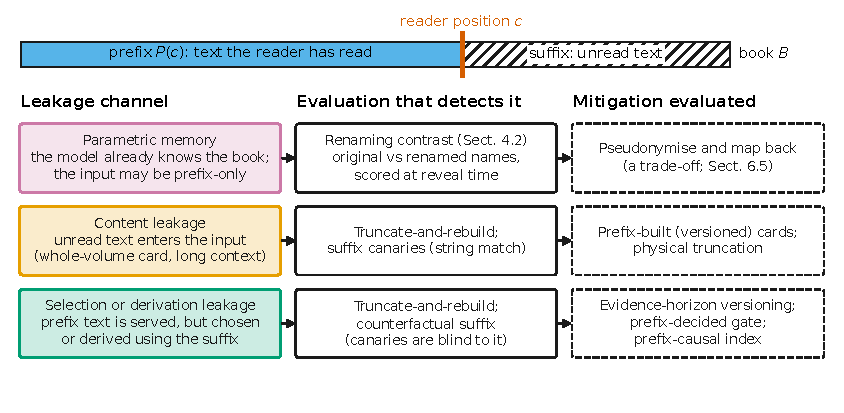
\includegraphics[width=\textwidth]{figures/fig1_channels.pdf}
\caption{Reader-faithfulness and the three leakage channels studied. The bar is a book $B$ split at reader position $c$ into the prefix $P(c)$ and the unread suffix. Each row names a channel, the evaluation that detects it in this paper, and the mitigation evaluated against it (dashed boxes). Suffix canaries are invented tokens planted after $c$; a counterfactual suffix rewrites the text after $c$ while keeping $P(c)$ byte-identical.}\label{fig:channels}
\end{figure}

%% ===================================================================================================== 4
\section{Methodology}\label{sec:method}

The study has two experimental tracks that share the reader-position and evidence-horizon concepts (Figure~\ref{fig:workflow}). Track 1 measures parametric memory with reveal-time events from public-domain novels (Sections~\ref{sec:m-corpus} and \ref{sec:m-memory}). Track 2 audits a narrative knowledge graph and generic assistant designs for future dependence (Sections~\ref{sec:m-pipeline} and \ref{sec:m-mitigation}); its generic-assistant experiments reuse Track 1's events.

\begin{figure}[!t]
\centering
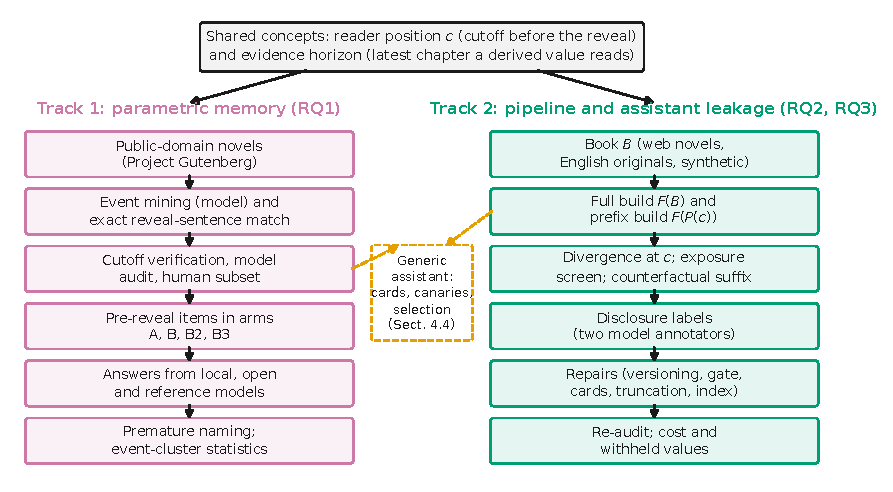
\includegraphics[width=\textwidth]{figures/fig2_workflow.pdf}
\caption{Workflow of the two research tracks. Track 1 (parametric memory, RQ1) builds reveal-time events from public-domain novels and compares premature naming across arms A (original names), B and B2 (two letter ciphers) and B3 (cue-preserving pseudonyms). Track 2 (pipeline and assistant leakage, RQ2 and RQ3) compares a full build $F(B)$ with a prefix build $F(P(c))$, labels divergences, applies repairs and re-audits. The dashed box marks the generic-assistant experiments, which use Track 1's events and Track 2's prefix-versus-full contrast.}\label{fig:workflow}
\end{figure}

\subsection{Corpus and Reveal-Time Event Construction}\label{sec:m-corpus}

All events come from Project Gutenberg plain-text novels \cite{gutenberg} first published before 1928. Texts are normalised by removing the Project Gutenberg header and footer (everything before the \texttt{*** START} marker and after the \texttt{*** END} marker) and carriage returns; no other change is made. Matching is whitespace-insensitive: a sentence is converted into a regular expression in which every run of whitespace matches any run of whitespace, so the line wrapping of the plain text does not affect it.

An event specifies a book, one or more alias surfaces, an identity name, a cast list of seven to nine names including the identity, a verbatim reveal sentence and a cutoff anchor. The reveal sentence must occur exactly once in the book; an event whose sentence occurs more than once or not at all is rejected rather than disambiguated. The cutoff is the start of the nearest chapter heading before the reveal. Because headings also appear in tables of contents, the last match of the heading pattern that begins before the reveal is used. When the alias does not occur before that heading, a fixed phrase position at least 200 characters before the reveal is used instead. A deterministic verifier then requires that the cutoff precede the reveal; that the alias occur at least three times before the cutoff; that no sentence before the cutoff contain both an alias surface and a capitalised token of the identity name; that the identity and the aliases share no capitalised token, so the name gives no lexical cue; and that the prefix contain enough cast mentions for the plain controls of Section~\ref{sec:m-memory}.

Candidate events are proposed by language models and then verified by these rules. For the exploratory sets (PD v2, v3 and v6) a model drafter proposed events book by book. For the confirmatory set, a pre-registered pipeline matched a fixed list of reveal-cue patterns (for example ``was none other than'', ``under the assumed name'', ``revealed himself'') in sentences of books sampled by fame band, and an open model extracted the alias, identity and reveal sentence, which had to be a verbatim substring of the passage. An auditor model from a different family labelled each reveal \textsc{explicit}, \textsc{implied} or \textsc{not supported} for the claim ``alias is identity''; \textsc{explicit} events form the confirmatory primary set. The exploratory events were audited after the fact by the commercial reference model, which labelled 20 of the 31 v2 and v3 events \textsc{explicit}, 2 \textsc{implied} and 9 \textsc{not supported}.

The resulting oracle is a \emph{reproducible, text-grounded oracle with model-assisted event selection}. Matching and cutoff verification are deterministic once an event has been proposed: anyone with the same texts and rules obtains the same items and labels. Which events exist, and whether a reveal sentence really identifies the alias, rest on model judgements. The oracle also fixes only what the book \emph{states}; an explicit reveal sentence is not the first point at which an attentive reader could infer the identity.

To validate the oracle, three authors labelled a stratified, seeded subset of 36 events: 18 exploratory events stratified by dataset, and 18 from the confirmatory primary set, including every high- and mid-fame event. Each event was labelled independently by two annotators, blind to all model labels, in an annotation tool that shows the reveal sentence in context and the same pre-reveal passages the models saw. For each event, annotators recorded whether they knew the book's plot; whether the reveal sentence identifies the alias explicitly, only implicitly or not at all; whether it reads as a revelation or as a reminder; whether a first-time reader of the earlier passages could name the identity (no, suspect, confident); and whether the event is valid. Agreement is summarised with Fleiss' $\kappa$ \cite{fleiss1971measuring}, and the headline gaps are recomputed without events that either annotator flagged. The annotators are three of the authors; they were blind to every model label but not to the study's hypotheses. Results are reported in Section~\ref{sec:r-memory}.

\subsection{Parametric-Memory Intervention and Controls}\label{sec:m-memory}

Each pre-reveal item shows the last 1,200 characters of text ending at the end of the sentence that contains the sampled alias mention, with the mention marked by double brackets. Up to eight pre-reveal mentions per event (four in the confirmatory study) are sampled at evenly spaced positions over the prefix, so items range from a few hundred to several hundred thousand characters before the cutoff. The candidate list is the event's cast in a seeded random order plus \textsc{undetermined}; the model answers with one letter, constrained to the allowed set by a JSON schema where the runtime supports it. Two kinds of control item use the same window construction. \emph{Post-reveal items} (alias mentions after the reveal, where the identity is the correct answer) check that the task is answerable, and \emph{plain controls} (mentions of ordinary cast members before the cutoff, where that member is the correct answer) measure how well the model reads the passage in each arm.

The arms differ only in names. Arm A shows the original text. Arm B replaces every proper-noun token, defined as a capitalised token of three or more letters that never occurs in lowercase in the book, by a case- and length-preserving letter substitution drawn with a fixed seed for each book. Honorifics and other protected words are unchanged, substitutions that collide with existing words are re-drawn, and the same mapping is applied to the window, the marked mention and the candidate list, so the correct letter is identical across arms. Arm B2 repeats B with a second, independent seed, and the analysis averages B and B2 so that a gap produced by one cipher alone is not counted. Arm B3 keeps the cues that a cipher destroys: the cast and alias name tokens are replaced by natural pseudonyms matched in gender (inferred from the pronouns that follow the name in the book) and in name type (given name or surname), while every other proper noun keeps the arm-B cipher, so that places and bystanders still give no memory cue. Because answers are letters, mapping an answer back to an identity is a lookup of that letter in the event's candidate list. Window text and candidate order are identical across arms.

Two probes measure memory directly. A closed-book probe asks who the alias is with no passage, and a title-assisted probe gives only the book title and the alias. The title-assisted probe defines the familiarity measure used in Section~\ref{sec:r-cue}: the number of five local models that name the identity. A validity gate, applied per model and dataset before any gap is interpreted, requires the two ciphers to agree on at least 90\% of plain controls, and the original and cipher arms to agree on at least 80\% of items from synthetic stories with invented names, where memory is impossible. Where pseudonyms restore control accuracy but leave the gap unchanged, we describe name-keyed memory as the most consistent explanation, not as a mechanism demonstrated inside the model.

\subsection{Pipeline Audit and Counterfactual Suffix Tests}\label{sec:m-pipeline}

The audited system is a narrative knowledge graph built for long web serials. It processes a volume as a whole and records three time axes per fact: discourse order, story time and \emph{knowledge time}, the position from which a reader could know the fact. Its reader query returns, for a character and position $c$, the latest value of each trait stamped at or before $c$. Because the volume is processed whole, the time at which a fact is written says nothing about when a reader could know it; knowledge time has to be reconstructed from where the evidence lies. We audit the \emph{persona stage}, which derives a character's gender, age band, speech register and archetype from the first twelve chapters in which the character appears, and stamps each trait at the chapter of first appearance. For a character first seen in chapter 1 whose pronouns appear only in chapter 3, a query at chapter 2 is served a gender that a build over chapters 1 and 2 would not hold.

\emph{Truncate-and-rebuild.} For a cut $k$, the persona stage is run on the full volume and, separately, on a copy of the database from which every chapter, span, mention and segment after $k$ has been deleted. Both builds start from the same stored mention-to-entity assignment, which isolates the persona stage from entity resolution. For every character with a persona fact in both builds, the values served at position $k+0.5$ are compared. The audit uses three translated web serials (\emph{Lord of the Mysteries}, \emph{Omniscient Reader's Viewpoint} and \emph{Reverend Insanity}): thirteen cuts give 289 character-cuts, and eleven further cuts give 396 more. Cuts are nested within a serial, so character-cuts are not independent.

\emph{Static exposure screen.} The evidence horizon of each trait was read from the stage's code (gender, for example, reads the first twelve attested chapters), and a fact is flagged as exposed at $k$ if its stamp is at most $k$ and its horizon exceeds $k$. The screen identifies where divergence is possible without rebuilding. Because the dependency table was read from the audited code, its soundness is close to true by construction, and we use it to certify safe cuts rather than to predict divergence.

\emph{Disclosure labels.} Divergence alone does not show that a reader is spoiled. For each divergent character-cut, two model annotators judged whether the full-build value was supported by the text up to the cut. Annotator 1 was the coding-assistant session that also implemented the repair, with labels written blind to all system values and frozen by hash. Annotator 2 was the commercial reference model with a fixed prompt and a quote check, under which an answer counts only if at least 80\% of its quoted words occur in order in the cited passage. A third reading with a permissive prompt brackets the rate. No human labelled these cuts, because the serials are copyrighted and were not shared beyond the project.

\emph{Counterfactual suffix.} Chapters up to $k$ are kept byte-identical, the gendered pronouns of every later span are swapped, the whole volume is rebuilt, and we ask whether the value served at $k$ changes. This tests dependence rather than divergence, needs neither truncation nor labels, and applies to closed-vocabulary outputs in which a planted string could never appear.

Two further instruments check the mechanism and its generality. The first is a synthetic volume of 40 chapters and 80 characters with known genders and a known chapter at which each character's own pronoun cue first appears, in nine configurations of cue density with five seeds each. The second is a pair of English public-domain originals (\emph{Oliver Twist} and \emph{The Three Musketeers}) passed through the unchanged stage. The stage's language-model path, which calls a local model for characters with at least 25 mentions, is audited separately.

\subsection{Leakage Mitigations and Generic-Assistant Experiments}\label{sec:m-mitigation}

All mitigations implement one principle: no value visible at position $c$ may be computed from evidence after $c$. They differ in where the principle is enforced.

\emph{Evidence-horizon versioning} (EHV) recomputes, for each attested chapter $c$, the deterministic profile from the evidence and cumulative mention counts of chapters up to $c$, and writes only the keys whose value changed, stamped at $c$. The reader query already returns the latest-stamped value per key, so the value served at $k$ equals what a build over chapters up to $k$ holds; body bindings carry a matching \texttt{confirmed\_at} stamp. \emph{The anchored pronoun cue} addresses a side effect of EHV, which withholds values whose pronouns settled early: it reads the first third-person pronoun after each mention within the mention's own narration span and is used only where the paragraph-level rule returns \emph{unknown}. Its setting was chosen by leave-one-serial-out selection and scored on the held-out serial. \emph{The prefix-decided gate} replaces the whole-volume mention count that decided whether the language model was called for a character with a count over the chapters read so far. The naive alternative evaluated against these repairs is \emph{hiding every exposed fact}.

For generic assistants, three designs are compared with reader-faithful counterparts on the confirmatory events, at a pre-registered cut just before the reveal chapter.

\emph{Whole-volume against versioned character cards.} A generator writes a card of at most 80 words for the aliased character from up to 12 passages spaced over the alias's mentions. The whole-volume build W draws mentions from the whole book; the prefix build P draws only mentions before the cut and clips every passage at the cut. P is the truncate-and-rebuild reference and equals a card versioned by evidence horizon. Each build runs on original names and under a frozen letter cipher. Because no model has seen the cipher names, a leak in renamed W cards can only come through the input, and renamed P cards should never leak, which serves as a validity check. A card leaks if it tells the reader at the cut who the alias is. The \emph{text rule} counts a leak when the card contains a name token of the identity that never occurs in the prefix; it is deterministic but applies only to the 19 events whose identity name first appears at the reveal. The \emph{judge rule} asks a fixed judge model, outside the generator set, whether the card states or clearly implies that alias and identity are the same person; it applies to all 54 events with alias mentions on both sides of the reveal. The two rules measure different things on different event sets and are never pooled. A robustness arm repeats W with an explicit instruction not to reveal spoilers.

\emph{Suffix canaries and long context.} Only the suffix is changed. Each identity name token after the cut is replaced by a fresh invented token, so the book still reveals the alias but under a name no model has seen, and one sentence ``\emph{alias} had been born in \emph{invented place}.'' is planted after the first post-reveal alias mention. A hit is an exact string match of a planted token in the output; it has no false positives and no memory explanation. The canary is applied to the W card (against the P card) and to a long-context assistant told where the reader is. Its input is up to 24,000 characters before the cut, the line \texttt{[READER POSITION: the reader has read up to here]}, and up to 16,000 characters after it (containing the reveal), with the instruction to answer from the text before the marker and not to reveal anything after it. The question is ``Who is \emph{alias}?''. The control is \emph{physical truncation}: the same prompt with the suffix removed. The harness is valid only if the P-card and truncated cells never hit.

\emph{Alias-merged against prefix-built retrieval.} A canary cannot see a leak that moves no suffix text. The selection test uses events whose identity is already named in the reader's prefix. At index time a resolver model reads the reveal window and decides whether alias and identity are one person. Retrieval for the alias then returns up to 12 passages spaced over the pre-cut mentions of both names, each clipped at the cut (asserted in code), and the card prompt runs on cipher names so that memory cannot contribute. The reference is a \emph{prefix-causal index} built from the prefix only, which has no reveal to merge on. Leakage here is labelled by the judge model, which was validated against the text rule only on events where that rule applies. The selection test is therefore the least-validated use of the judge: both names occur in the input, which is where a judge is most needed.

\emph{Pseudonymise and map back}, the memory mitigation, replaces the names in the input with pseudonyms, runs the model and maps names in the answer back. It was pre-registered with a non-inferiority margin of 5 points on accuracy after the reveal and on plain controls.

%% ===================================================================================================== 5
\section{Experimental Setup}\label{sec:setup}

\emph{Datasets and splits.} Table~\ref{tab:data} lists every dataset by track. The exploratory memory sets are PD v2 (19 events), v3 (12 events from new books) and v6 (7 events from new books). A further set, v7 (9 events, local models only), was a prospective familiarity contrast that proved inconclusive and is reported in the supplementary material. The confirmatory set has 68 events from 65 books, split by book into development and test; its primary set is the 32 test events audited \textsc{explicit} (25 from low-fame, 6 from mid-fame and 1 from a high-fame book, by the number of Wikipedia language editions linked from the book's Wikidata item \cite{vrandecic2014wikidata}). No book appears in more than one memory set. The card, canary and selection experiments reuse the confirmatory events and are therefore not independent of the confirmatory memory study; the pipeline audit uses separate corpora.

\begin{table}[!t]
\caption{Datasets by track. For the memory sets, ``Items'' are pre-reveal / post-reveal / plain-control items. All events are model-selected and verified by exact search; the synthetic volume is generated with known truth.}\label{tab:data}
\footnotesize
\begin{tabular*}{\textwidth}{@{\extracolsep\fill}p{2.2cm}p{3.3cm}p{3.0cm}p{2.8cm}}
\toprule
Set & Events or units & Items or comparisons & Role \\
\midrule
\multicolumn{4}{l}{\emph{Track 1: parametric memory}} \\
PD v2 & 19 events, 19 books & 135 / 30 / 152 & Exploratory \\
PD v3 & 12 events, 12 new books & 96 / 24 / 96 & Exploratory replication \\
PD v6 & 7 events, 7 new books & 54 / 14 / 56 & Exploratory replication \\
Confirmatory & 68 events, 65 books; 53 test, 32 primary & 260 / 57 / 136 (all 68 events) & Pre-registered confirmation \\
Unseen stories & 17 model-written stories & as confirmatory & Negative control \\
\midrule
\multicolumn{4}{l}{\emph{Track 2: pipeline and generic assistants}} \\
Web serials & 3 serials; 13 + 11 cuts & 289 + 396 character-cuts & Persona-stage audit \\
English originals & 2 novels & 179 character-cuts & Transfer check \\
Synthetic volume & 40 chapters, 80 characters; 9 configurations, 5 seeds & 1,240 pairs per configuration & Known-truth check \\
Character cards & 54 events (judge), 19 (text rule) & 4 cells per event and model & Content leak \\
Suffix canaries & 54 (cards), 46 (long context) events & with and without suffix & Content leak \\
Selection & 36 events, 24 merged & merged vs prefix index & Selection leak \\
\midrule
\multicolumn{4}{l}{\emph{Human validation}} \\
Reveal check & 36 events (18 exploratory, 18 confirmatory) & 72 labels, 2 per event & Oracle validation \\
\botrule
\end{tabular*}
\end{table}

\emph{Models and execution.} Table~\ref{tab:models} lists the models. Local models ran through ollama \cite{ollama} on a laptop GPU (NVIDIA RTX 4060, 8\,GB) at temperature 0 with a fixed seed. The confirmatory open models were served with vLLM \cite{kwon2023vllm} on one rented NVIDIA L40S GPU (48\,GB) \cite{runpod2026pricing}, also at temperature 0. The commercial reference model was called through its vendor API \cite{openai2026models} with reasoning disabled. It is used as a \emph{positive control}: if name-keyed memory exists for a strong model on familiar books, a valid harness must detect it. It never decides what is true, and it is kept separate from the open models in every analysis. A fourth confirmatory arm (Claude Sonnet 5.5 through a command-line interface \cite{anthropic2026claudecode}) stopped at a usage limit after 211 of 1,218 planned answers. It is an incomplete arm, excluded from every pooled estimate and described only in the supplementary material.

\begin{table}[!t]
\caption{Models, builds and execution settings. Local builds are ollama quantisations; temperature 0 throughout.}\label{tab:models}
\footnotesize
\begin{tabular*}{\textwidth}{@{\extracolsep\fill}p{3.3cm}p{1.5cm}p{2.6cm}p{3.9cm}}
\toprule
Model (reference) & Build & Context, hardware & Used for \\
\midrule
Qwen2.5-7B-Instruct \cite{qwen2025qwen25} & Q4\_K\_M & 2K--12K tokens; RTX 4060 & Memory; cards; canaries; selection; resolver; persona path \\
Llama-3.1-8B-Instruct \cite{grattafiori2024llama3} & Q4\_K\_M & as above & Memory; cards; canaries; selection \\
Mistral-7B-Instruct \cite{jiang2023mistral} & Q4\_K\_M & as above & Memory; cards; canaries; selection \\
Gemma-2-9B \cite{gemma2024gemma2} & Q4\_0 & 2K tokens; RTX 4060 & Memory \\
Phi-4-mini \cite{microsoft2025phi4mini} & Q4\_K\_M & 2K tokens; RTX 4060 & Memory \\
Qwen3-8B \cite{qwen2025qwen3} & Q4\_K\_M & RTX 4060 & Judge (cards, selection) \\
\midrule
Qwen2.5-32B-Instruct \cite{qwen2025qwen25} & AWQ 4-bit & vLLM; L40S & Confirmatory memory; event mining; larger cards \\
OLMo-2-32B-Instruct \cite{olmo2024olmo2} & fp8 & vLLM; L40S & Confirmatory memory; second judge \\
Mistral-Small-3.2-24B \cite{mistral2025small32} & fp8 & vLLM; L40S & Confirmatory memory; event audit; larger cards \\
\midrule
gpt-5.6-luna \cite{openai2026models} & API & vendor service & Positive control; exploratory event audit; disclosure annotator 2 \\
\botrule
\end{tabular*}
\end{table}

\emph{Metrics.} Table~\ref{tab:metrics} defines each reported metric and states whether it is computed by deterministic matching or depends on a model judgement.

\begin{table}[!t]
\caption{Metrics. ``Deterministic'' means computed by exact matching against text or stored system values, with no model judgement.}\label{tab:metrics}
\footnotesize
\begin{tabular*}{\textwidth}{@{\extracolsep\fill}p{3.1cm}p{6.5cm}p{2.3cm}}
\toprule
Metric & Definition & Evidence type \\
\midrule
Original-minus-cipher gap & $\Delta_{AB}$ in Eq.~\eqref{eq:gap}: premature naming under A minus the mean of B and B2 & Deterministic \\
Original-minus-pseudonym gap & $\Delta_{AB3}$: the same with arm B3 & Deterministic \\
Recovered fraction & $\rho=(p_{B3}-p_B)/(p_A-p_B)$ & Deterministic \\
Post-reveal accuracy & Share of post-reveal items answered with the identity & Deterministic \\
Pipeline divergence & Share of character-cuts whose served value differs between full and prefix builds & Deterministic \\
Suffix dependence & Share of cuts whose served value changes under a counterfactual suffix & Deterministic \\
Genuine disclosure & Share of character-cuts with a divergent value unsupported by the prefix & Model annotators \\
Card leak, text rule & The card contains an identity token absent from the prefix & Deterministic \\
Card leak, judge rule & The judge says the card identifies the alias with the identity & Model judge \\
Canary rate & The output contains a token planted after the cut & Deterministic \\
Selection leak & Judge rule applied to cards built from alias-merged retrieval & Model judge \\
Human reveal check & Two author-annotators per event judge explicitness, inferability and validity & Human \\
Runtime & Wall-clock time of a stage or run on the stated hardware & Measured \\
\botrule
\end{tabular*}
\end{table}

\emph{Statistical protocol.} Items within an event share a book, a reveal and often a passage, so the event is the resampling unit throughout. Intervals for gaps are 95\% percentile intervals from an event-cluster bootstrap \cite{efron1993bootstrap,dror2018hitchhiker}, with 5,000 resamples (seed 20261019) in the exploratory analyses and 10,000 (seed 20261101) in the confirmatory analysis. When several models are pooled in the exploratory analysis, their items are concatenated within events before events are resampled, so the pooled interval keeps the dependence between a model's items and between models on the same event. Exploratory analyses report two-sided exact sign tests over events. The confirmatory hypotheses were one-sided at $\alpha=0.05$, with a Holm correction \cite{holm1979simple} over the family \{H1, H2, H3, H5\} at the pre-registered family-wise level. The confirmatory pooled gap (H1) combines the per-model event-weighted estimates in a DerSimonian--Laird random-effects model \cite{dersimonian1986meta} with a Hartung--Knapp interval \cite{hartung2001tests}. Random effects are used because the three models are treated as a sample of plausible open models whose true gaps may differ; the pooled value estimates their average, not the behaviour of any one model. Familiarity associations use Spearman's $\rho$ with a permutation $p$-value. Proportions in the pipeline audit carry Wilson intervals \cite{wilson1927probable}; because cuts are nested, these intervals are optimistic. The confirmatory study's rules, prompts, events and thresholds were written and hashed before the data they govern were collected \cite{nosek2018preregistration}, and an incomplete model run is excluded from pooled tests and reported separately. An earlier version of the exploratory analysis treated items as independent; switching to event resampling widened the intervals, and every result here uses event resampling.

\emph{Reproducibility.} Every number in this paper is recomputed from stored result files by scripts in the project repository (see Declarations), and a consistency script checks that each value quoted in the manuscript matches its source. Pre-registrations and event manifests are hashed. Project Gutenberg texts are public domain and can be re-downloaded by the identifiers listed in the supplementary material. The three web serials are copyrighted and are not redistributed, so the audit on them can be reproduced only with the same texts. Timings are wall-clock measurements on the stated hardware; local and rented GPU timings describe the cost of these experiments and are not a controlled hardware benchmark.

%% ===================================================================================================== 6
\section{Results}\label{sec:results}

\subsection{Parametric-Memory Leakage}\label{sec:r-memory}

\emph{Exploratory study.} Figure~\ref{fig:forest} and Table~\ref{tab:explor} report the leakage gap per model and dataset. For the reference model the gap was positive in all three exploratory datasets: $+35.2$ points [$+20.2$, $+50.0$] on v2, $+18.2$ [$+4.2$, $+33.9$] on v3 and $+16.7$ [$+5.4$, $+28.6$] on v6. Pooled over all 38 events it was $+26.0$ points [$+16.8$, $+36.0$], with 22 events positive, 1 negative and the rest tied (sign test $p=1\times10^{-5}$). The pooled value is the item-pooled estimate of Eq.~\eqref{eq:gap} over the 285 pre-reveal items (135, 96 and 54 in the three datasets); it equals the item-weighted average of the three dataset gaps, which is why it lies above their unweighted mean. Restricted to the 20 events that the post hoc label audit marked \textsc{explicit}, the reference model's gap was $+29.9$ [$+15.0$, $+45.8$]. For the four local models that passed the validity gate, the pooled gap was $+11.5$ [$+4.5$, $+19.0$] over 38 events (sign test $p=0.05$), but on the seven v6 books it was $-5.9$ [$-14.8$, $+1.0$], with 1 event positive and 4 negative. The pre-registered replication on v6 therefore failed for the small local models and held for the reference model.

\begin{figure}[!t]
\centering
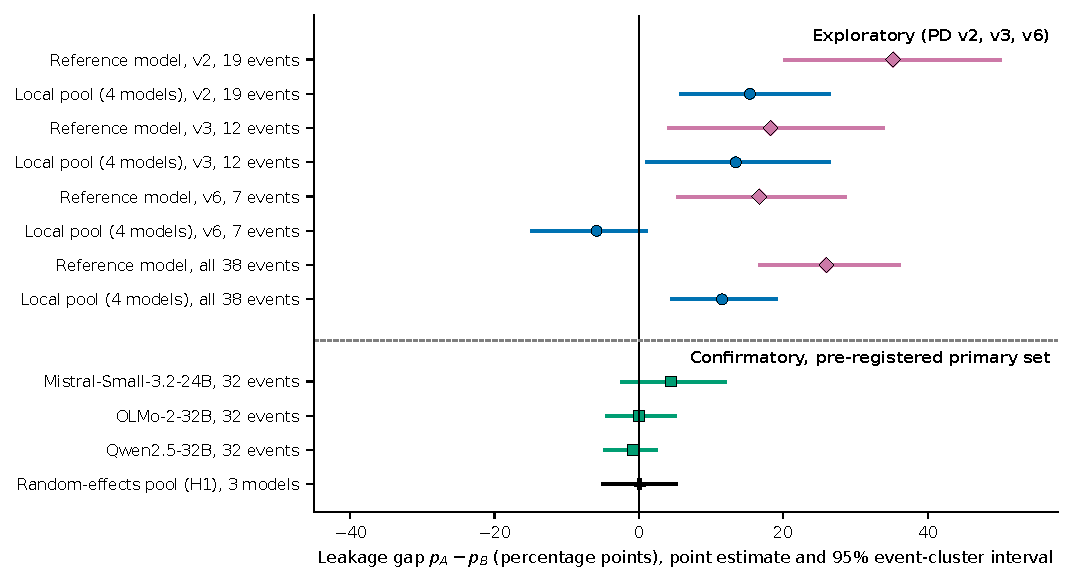
\includegraphics[width=\textwidth]{figures/fig3_forest.pdf}
\caption{Leakage gap $p_A-p_B$ (premature naming under original names minus the mean of two letter ciphers, in percentage points) with 95\% event-cluster bootstrap intervals. Upper block: exploratory datasets (item-pooled estimates); the local pool concatenates the items of the four models that passed the validity gate. Lower block: pre-registered confirmatory study on the 32-event primary set (event-weighted estimates) and the random-effects pool of the three open models (H1, Hartung--Knapp interval).}\label{fig:forest}
\end{figure}

\begin{table}[!t]
\caption{Exploratory leakage gap per model and dataset, in points with 95\% event-cluster intervals (item-pooled estimator; 5,000 event resamples with the same seed for every cell).}\label{tab:explor}
\footnotesize
\begin{tabular*}{\textwidth}{@{\extracolsep\fill}lccc}
\toprule
Model & v2 (19 events) & v3 (12 events) & v6 (7 events) \\
\midrule
Reference model (gpt-5.6-luna) & $+35.2$ [$+20.2$, $+50.0$] & $+18.2$ [$+4.2$, $+33.9$] & $+16.7$ [$+5.4$, $+28.6$] \\
Gemma-2-9B & $+13.0$ [$+1.8$, $+25.9$] & $+25.0$ [$+4.7$, $+47.9$] & $-12.0$ [$-29.6$, $-1.8$] \\
Llama-3.1-8B & $+14.1$ [$+3.2$, $+27.7$] & $+14.6$ [$+3.6$, $+27.1$] & $-15.7$ [$-40.7$, $+4.5$] \\
Mistral-7B-Instruct & $+24.1$ [$+12.4$, $+37.5$] & $+9.9$ [$-5.2$, $+24.0$] & $+1.8$ [$-8.0$, $+13.0$] \\
Phi-4-mini & $+10.4$ [$+0.8$, $+22.5$] & $+4.2$ [$-6.2$, $+17.2$] & $-3.7$ [$-14.4$, $+4.6$] \\
Qwen2.5-7B & $+22.2$ [$+9.8$, $+35.9$] & $+9.9$ [$-3.6$, $+24.5$] & $+0.0$ [$-16.1$, $+14.3$] \\
\botrule
\end{tabular*}
\end{table}

\emph{Confirmatory study.} The pre-registered study tested the effect on 68 new events from 65 books with three open models. Each model answered 2,220 questions: the 453 items of all 68 events in four arms (A, B, B2 and B3; 1,812 answers), and the closed-book and title-assisted probes for each event in three arms (204 answers each). The primary analysis uses only the pre-reveal items of the 32 primary test events. Table~\ref{tab:confirm} reports the per-model gaps and the pre-registered tests. No model showed a gap added by original names: $+4.4$ points [$-2.3$, $+12.0$] for Mistral-Small-3.2-24B, $+0.0$ [$-4.4$, $+4.9$] for OLMo-2-32B and $-0.8$ [$-4.7$, $+2.3$] for Qwen2.5-32B. The random-effects pool was $+0.1$ [$-5.0$, $+5.2$] (H1, one-sided $p=0.47$). The primary familiarity contrast (P1), the gap of high- and mid-fame events minus that of low-fame events, pointed in the expected direction ($+7.6$ points [$-1.4$, $+18.3$], one-sided $p=0.059$), but the design could detect only differences of about 12.8 points with 80\% power, so it is inconclusive. The correlation between fame and gap (H3, $\rho=+0.30$ over 32 events) met its raw criterion but not the Holm-corrected one (adjusted $p=0.145$). In the closed-book probe each model named the hidden identity in only 2 of 68 events. Excluding the two primary events whose mined ``identity'' is a descriptive phrase rather than a name (a post hoc check with a fixed rule) gave $-1.1$ [$-3.8$, $+1.6$]. The unseen-story control (17 model-written stories) gave gaps of exactly zero for all three models; a recap task produced no spoiler in 144 outputs per condition; and a check of 62 books against a public index of the OLMo~2 pretraining corpus found no association between a book's presence and its gap (Spearman $+0.13$, $p=0.41$).

\begin{table}[!t]
\caption{Confirmatory study (pre-registered; primary set of 32 test events; event-weighted estimates; 10,000 event resamples). The incomplete fourth arm is excluded. MDD: minimum detectable difference at 80\% power.}\label{tab:confirm}
\footnotesize
\begin{tabular*}{\textwidth}{@{\extracolsep\fill}p{4.4cm}p{4.6cm}p{2.4cm}}
\toprule
Quantity & Estimate [95\% interval] & Decision \\
\midrule
Mistral-Small-3.2-24B, $\Delta_{AB}$ & $+4.4$ [$-2.3$, $+12.0$] & -- \\
OLMo-2-32B, $\Delta_{AB}$ & $+0.0$ [$-4.4$, $+4.9$] & -- \\
Qwen2.5-32B, $\Delta_{AB}$ & $-0.8$ [$-4.7$, $+2.3$] & -- \\
\midrule
H1: pooled $\Delta_{AB}$, 3 models & $+0.1$ [$-5.0$, $+5.2$]; $p=0.47$ & Not supported \\
H2: pooled $\Delta_{AB3}$ & $+5.7$ [$-1.3$, $+12.6$] & Not supported \\
P1: high/mid minus low fame & $+7.6$ [$-1.4$, $+18.3$]; $p=0.059$; MDD 12.8 & Inconclusive \\
H3: fame against gap (Spearman) & $+0.30$; Holm-adjusted $p=0.145$ & Not confirmed \\
H5: pseudonymise and map back & premature naming 5.0\% to 2.6\%; post-reveal accuracy $-6.7$ & Margin not met \\
\botrule
\end{tabular*}
\end{table}

The confirmatory null does not contradict the exploratory finding. The confirmatory sample is dominated by low-familiarity books (25 of 32 primary events), and the closed-book probe indicates that the open models hold little memory of them, whereas the exploratory books include several of the best-known novels in English. The pattern is consistent with a familiarity-dependent effect (Section~\ref{sec:r-cue}). Familiarity was not manipulated, however, the contrast that would test it was underpowered, and the two studies also differ in models and in event-mining procedure, so these alternative explanations are not excluded.

\emph{Human validation of the oracle.} Both annotators judged the reveal sentence an explicit identification in 34 of the 36 validated events (94.4\%, Wilson [81.9, 98.5]\%); in the remaining two, one or both annotators judged it implied only, and no annotator judged that a reveal failed to identify the alias. Every validated event that the model audit had labelled \textsc{explicit} (28 of 28; Wilson lower bound 87.9\%) was confirmed as explicit by both annotators. No annotator judged a hidden identity confidently inferable from the pre-reveal passages (0 of 36 events, Wilson upper bound 9.6\%), but at least one annotator suspected it from clues in 17 of 36 events, and both did in 8. In 9 events one annotator read the reveal as a reminder of something already stated rather than as a revelation; the other annotator disagreed in each case. One annotator judged 6 of the 18 validated confirmatory events invalid, and the other annotator accepted all six; no exploratory event was flagged. Raw agreement was 97.2\% on whether the reveal is explicit (Fleiss $\kappa=0.65$) and 75.0\% on inferability ($\kappa=0.45$). For the validity and revelation questions one answer dominates, which makes $\kappa$ uninformative, so raw agreement (83.3\% and 75.0\%) is the better summary. The annotators knew the book's plot in 1 of 72 labels. Recomputing the main estimates on the validated events changed no conclusion. The reference model's exploratory gap was $+27.4$ [$+16.0$, $+40.3$] on the 18 validated exploratory events, none of which was flagged. The confirmatory pooled gap was $-1.2$ [$-6.3$, $+3.9$] on the 18 validated confirmatory events and $-3.9$ [$-5.9$, $-1.9$] after removing the six events one annotator flagged (12 events), so no positive gap appears in either case.

\subsection{Cue-Preserving Controls and Book Familiarity}\label{sec:r-cue}

The letter cipher lowered plain-control accuracy relative to original names (for Qwen2.5-7B on v2, from 95.4\% to 80.3\%), so part of an original-minus-cipher gap could in principle reflect lost reading cues rather than memory. Cue-preserving pseudonyms restored control accuracy to the original level (96.7\% for the same model; all models in the supplementary material). They did not remove the leakage gap (Figure~\ref{fig:cue} and Table~\ref{tab:cue}). Pooled over the 31 v2 and v3 events for the models that passed the validity gate, the gap was $+14.6$ [$+7.0$, $+22.7$] against the cipher and $+16.1$ [$+8.2$, $+25.0$] against pseudonyms, and the recovered fraction was $-0.11$ [$-0.36$, $+0.06$]. The pre-registered decision rule classed a recovered fraction below one third as memory-dominant, and the whole interval lies below that line, so restoring name cues recovers at most a small share of the gap. The interval includes zero and small negative values; the point estimate should be read as ``near zero'', not as evidence that pseudonyms increase leakage.

\begin{figure}[!t]
\centering
\includegraphics[width=\textwidth]{figures/fig4_cue_preserving.pdf}
\caption{Cue-preserving control. Leakage gaps on the 19 v2 events for each model, and pooled over the 31 v2 and v3 events for the models that passed the validity gate (right of the dashed line). A: original names; B: mean of two letter ciphers; B3: pseudonyms matched in gender and name type, with other proper nouns ciphered. Bars are 95\% event-cluster intervals. If lost name cues explained the A$-$B gap, the A$-$B3 gap would shrink towards zero.}\label{fig:cue}
\end{figure}

\begin{table}[!t]
\caption{Cue-preserving control pooled over the 31 v2 and v3 events (points, 95\% event-cluster intervals). Events A$>$B3 / A$<$B3: events in which original names gave more / less premature naming than pseudonyms.}\label{tab:cue}
\footnotesize
\begin{tabular*}{\textwidth}{@{\extracolsep\fill}p{2.5cm}cccc}
\toprule
Pool & $\Delta_{AB}$ & $\Delta_{AB3}$ & Recovered fraction & A$>$B3 / A$<$B3 \\
\midrule
Models passing the gate & $+14.6$ [$+7.0$, $+22.7$] & $+16.1$ [$+8.2$, $+25.0$] & $-0.11$ [$-0.36$, $+0.06$] & 19 / 8 \\
All six models & $+17.2$ [$+10.2$, $+24.6$] & $+18.8$ [$+11.6$, $+26.4$] & $-0.09$ [$-0.24$, $+0.02$] & 23 / 5 \\
\botrule
\end{tabular*}
\end{table}

\emph{Familiarity (post hoc).} After the v6 replication failed, we examined whether the gap varies with how well models recognise a book, measured as the number of the five local models that name the identity in the title-assisted probe (Figure~\ref{fig:dose}). For the valid local pool, the per-event gap correlated with recognition (Spearman $+0.59$, permutation $p=0.00015$, 38 events). The gap was near zero for books recognised by at most three of the five models ($+0.7$ [$-3.7$, $+5.5$] for 20 events recognised by none or one; $-0.4$ [$-8.2$, $+6.2$] for 6 recognised by two or three) and large for books recognised by four or five ($+30.3$ [$+15.3$, $+43.8$], 12 events). For the reference model the gap was positive in every group and larger for recognised books (Spearman $+0.37$, $p=0.024$). This analysis is post hoc, the groups are small (the six recognition levels contain 10, 10, 4, 2, 5 and 7 events), and for the local pool the predictor and the outcome come from the same models, so it is not an independent causal estimate. The pattern is consistent with the v6 replication having failed because its books are poorly recognised, without establishing familiarity as the cause.

\begin{figure}[!t]
\centering
\includegraphics[width=0.8\textwidth]{figures/fig5_familiarity_posthoc.pdf}
\caption{Post hoc familiarity analysis over the 38 exploratory events. Recognition is the number of five local models that name the hidden identity when given only the book title and the alias. Points are mean per-event gaps (A minus B, points) with 95\% bootstrap intervals over the events in each group; $n$ is the number of events per group. The predictor shares models with the local-pool outcome.}\label{fig:dose}
\end{figure}

\subsection{Pipeline Divergence and Evidence-Horizon Versioning}\label{sec:r-pipeline}

Table~\ref{tab:pipeline} consolidates the audit of the persona stage. Each row states its own denominator, and the cut sets are not interchangeable. On the original 13 cuts of the three web serials, the served value differed from a prefix-only build in 23 of 289 character-cuts (8.0\%, Wilson [5.4, 11.7]\%). On 11 added cuts it differed in 18 of 396 (4.5\%), giving 41 of 685 (6.0\%) over all 24 cuts. The same unmodified stage diverged in 8 of 179 character-cuts on two English public-domain originals. Every divergence on the original cuts was a gender value, together with the archetype string derived from it; age band and register never diverged. On the synthetic volume with known truth, the status quo diverged in 9.2\% to 17.1\% of 1,240 pairs per configuration, and the number of pairs served a known gender before the character's own cue existed fell as cue density rose (70, 17 and 4 pairs at densities 0.10, 0.35 and 0.70, without adversarial pronouns), which shows the mechanism and its dose--response without any annotator. Under evidence-horizon versioning the observed divergence was 0 in every reported test (0 of 289 cuts, Wilson [0, 1.3]\%; 0 of 685; 0 in each synthetic configuration). The entity resolver itself was prefix-causal: 0 of 28,165 mention--cut comparisons over 14 cuts changed entity when later chapters were removed.

\begin{table}[!t]
\caption{Persona-stage audit. Divergence: served value differs from a prefix-only build. Dependence: served value changes when only the suffix is rewritten. Disclosure: divergent value not supported by the prefix (model annotators). Character-cuts on nested cuts are not independent.}\label{tab:pipeline}
\footnotesize
\begin{tabular*}{\textwidth}{@{\extracolsep\fill}p{5.0cm}p{1.9cm}p{2.5cm}p{2.0cm}}
\toprule
Measurement (data) & Denominator & Status quo & With EHV \\
\midrule
Divergence, original 13 cuts (3 serials) & 289 cuts & 23 (8.0\%) & 0 \\
Divergence, 11 added cuts & 396 cuts & 18 (4.5\%) & 0 \\
Divergence, all 24 cuts & 685 cuts & 41 (6.0\%) & 0 \\
Divergence, English originals & 179 cuts & 8 (4.5\%) & 0 \\
Divergence, synthetic volume & 1,240 pairs each & 9.2--17.1\% & 0 \\
Divergence after hiding every exposed fact (naive repair) & 289 cuts & 82 (28.4\%) & -- \\
Suffix dependence, original cuts & 289 cuts & 47 (16.3\%) & 0 of 304 \\
\midrule
Genuine disclosure, annotator 2, all cuts & 685 cuts & 18 (2.6\%) & -- \\
Genuine disclosure, annotator 2, permissive prompt & 685 cuts & 14 (2.0\%) & -- \\
Genuine disclosure, original cuts, annotator 1 / 2 & 289 cuts & 5 (1.7\%) / 10 (3.5\%) & -- \\
\botrule
\end{tabular*}
\end{table}

\emph{Divergence is not disclosure.} Of the 41 divergent character-cuts, annotator 2 judged 18 genuine premature disclosures (2.6\% of 685 cuts, Wilson [1.7, 4.1]\%), 21 already supported by the text up to the cut, and 2 reversed (the status quo served \emph{unknown} where the prefix build held the correct value). With a permissive prompt the rate was 2.0\%; on the original 289 cuts annotator 1 gave 1.7\% and annotator 2 gave 3.5\%. All three readings exclude zero, and the defensible statement is a range of 1.7--3.5\% of character-cuts rather than a point estimate. The two annotators agreed with $\kappa=0.61$ on the 117 characters both labelled and never contradicted each other on male against female; both are models, and one of them implemented the repair.

\emph{Hiding is worse than nothing; versioning is faithful but not correct.} Hiding every exposed fact, the obvious way to make every stamp honest, diverged from a prefix build in 82 of 289 cuts, more than the 23 it started with: it removed the leaking values but also 80 values that the prefix build already held. In most exposed cuts the value had already settled in the prefix, because the coarse horizon (twelve attested chapters) is later than the chapter in which the pronouns fixed it. Table~\ref{tab:repair} shows what a reader is actually served. On 245 exposed cuts with a male or female reference label, versioning served the same values as a prefix-only build: 149 correct against 184 for the status quo, with 91 withheld against 56. It trades correctness for faithfulness by withholding values the prefix supports. On the held-out serial, the anchored pronoun cue recovered almost all of that loss (360 correct against 361 for the status quo and 326 for plain versioning, with 6 wrong against 5) while keeping divergence at zero. It did not transfer to the English originals, where its error rate (7.8\%) exceeded the pre-registered 3\% limit. All five wrong values in the upper block of Table~\ref{tab:repair} belong to one character in both builds, an extraction error unrelated to the cut.

\begin{table}[!t]
\caption{What the reader is served at exposed cuts. Correct: value matches the reference label; withheld: the system serves \emph{unknown}; wrong: the other gender. Reference labels combine the two model annotators.}\label{tab:repair}
\footnotesize
\begin{tabular*}{\textwidth}{@{\extracolsep\fill}p{6.4cm}ccc}
\toprule
Build & Correct & Withheld & Wrong \\
\midrule
\multicolumn{4}{l}{\emph{All web-serial cuts: 245 exposed cuts, 67 characters}} \\
Status quo & 184 (75.1\%) & 56 & 5 \\
Prefix-only build $=$ evidence-horizon versioning & 149 (60.8\%) & 91 & 5 \\
\multicolumn{4}{l}{\emph{Held-out serial evaluation: 512 pairs, 98 characters (pre-registered)}} \\
Status quo & 361 (70.5\%) & 146 & 5 \\
Plain versioning & 326 (63.7\%) & 181 & 5 \\
Versioning with the anchored pronoun cue & 360 (70.3\%) & 146 & 6 \\
\botrule
\end{tabular*}
\end{table}

\emph{Truncation is a sound but incomplete test.} The counterfactual suffix found 47 of the 289 original character-cuts (16.3\%) whose served gender changed when only later chapters changed, against the 23 that truncate-and-rebuild detected. All 23 divergent cuts were among the 47, and none of the 47 lay outside an exposure window. In 24 cuts the served value was right on this book only because later chapters happened to agree with earlier ones. Under versioning, 0 of 304 compared cuts changed.

\emph{The model path.} With the same prompt in both builds, the local model's discrete trait differed in 0 of 101 character-cut pairs, so later chapters did not change the model's reading at these settings. The gate that decided whether to call the model did depend on the future: because it used a whole-volume mention count, 50 of 296 pairs were served the model's reading in the full build and the deterministic one in the prefix build. Deciding the gate chapter by chapter removed all 50.

\subsection{Character Cards, Long Context, and Selection Leakage}\label{sec:r-assistant}

\emph{Whole-volume against versioned cards (content leakage).} Table~\ref{tab:cards} and Figure~\ref{fig:cards} compare the two builds. On cipher names, which no model has seen, the whole-volume card named the hidden identity before the reveal in 18.5\% of 54 events by the judge rule and in 24.6\% of 19 events by the text rule; the versioned card did so in 1.2\% and 0.0\%. The two percentages are different metrics on different event sets and are reported separately. The pre-registered input-channel contrast (W minus P, renamed) was $+17.3$ points [$+9.3$, $+26.5$] by the judge rule and $+24.6$ [$+8.8$, $+42.1$] by the text rule. The memory-only contrast, the versioned card on original names minus the same card on cipher names, was $+2.5$ points by the judge rule, so for these books and models the build, not the model's memory, was the larger source of leakage. Larger models (24--32B) showed the same pattern (whole-volume 23.1\% against versioned 1.9\%, judge rule). An explicit instruction to avoid spoilers did not remove the leak: the instructed whole-volume card still leaked in 14.8\% of events by the judge rule (difference from the versioned card $+14.8$ [$+5.6$, $+24.1$]) and in 15.8\% by the text rule, where the interval of the difference included zero ([$0.0$, $+31.6$]). Against the deterministic text rule on 380 card labels, the judge found 91.7\% of text-rule leaks and flagged 0.9\% of non-leaks ($\kappa=0.92$), and a second judge from another model family agreed with it on 97.8\% of 684 labels ($\kappa=0.88$). The judge's validity on the 35 events outside the text rule's scope is not established, and the judge-rule figures carry that limit.

\begin{table}[!t]
\caption{Cards naming the hidden identity before the reveal (\% of events), pooled over generators. W: whole-volume card; P: versioned, prefix-built card; orig, ren: original or cipher names. Input channel: W$-$P on cipher names (points, 95\% event-cluster interval).}\label{tab:cards}
\footnotesize
\begin{tabular*}{\textwidth}{@{\extracolsep\fill}p{3.6cm}ccccc}
\toprule
Rule, generators (events) & W orig & W ren & P orig & P ren & Input channel \\
\midrule
Text rule, 7--8B (19) & 31.6 & 24.6 & 0.0 & 0.0 & $+24.6$ [$+8.8$, $+42.1$] \\
Judge rule, 7--8B (54) & 19.1 & 18.5 & 3.7 & 1.2 & $+17.3$ [$+9.3$, $+26.5$] \\
Text rule, 24--32B (19) & 21.1 & 21.1 & 0.0 & 0.0 & $+21.1$ [$+5.3$, $+39.5$] \\
Judge rule, 24--32B (54) & 21.3 & 23.1 & 1.9 & 1.9 & $+21.3$ [$+13.0$, $+30.6$] \\
\botrule
\end{tabular*}
\end{table}

\begin{figure}[!t]
\centering
\includegraphics[width=\textwidth]{figures/fig6_cards.pdf}
\caption{Cards naming the hidden identity before the reveal, per generator, on cipher names. Left: judge rule (a fixed judge model; 54 events). Right: deterministic text rule (an identity token absent from the reader's prefix appears in the card; 19 events). Circles: whole-volume card (W); squares: versioned, prefix-built card (P); triangle: W with an explicit instruction to avoid spoilers (Qwen2.5-7B only). Models to the right of the dashed line are 24--32B.}\label{fig:cards}
\end{figure}

\emph{Suffix canaries (content leakage, deterministic).} Table~\ref{tab:canary} reports the canary experiments, which involve no judge. The whole-volume card quoted a token planted after the cut in 22.8\% of 54 events, against 0\% for the versioned card. The long-context assistant told where the reader is quoted a post-marker token in 40.6\% of 46 events, against 0\% when the suffix was physically removed. All three generators were positive in both designs, and no versioned or truncated cell ever produced a hit, which validates the harness. The leak was not specific to the identity: the planted birthplace sentence was carried into 21.0\% of whole-volume cards and 11.1\% of long-context answers.

\emph{Alias-merged retrieval (selection leakage, judge-dependent).} In 24 of the 36 events whose identity is named in the prefix, the resolver merged alias and identity using the reveal window. Retrieval then served only passages the reader had already read, yet cards built from them identified the alias with the identity in 19.4\% of merged events, against 1.4\% for the prefix-causal index (paired event-level difference $+18.1$ points [$+4.2$, $+33.3$]); all three generators were positive. A canary cannot detect this leak, because no suffix token enters the input, and a position filter on served passages passes it. Excluding the four merged events whose mined identity is a descriptive phrase (post hoc, fixed rule) gave $+18.3$ [$+3.3$, $+36.7$] over 20 events. The result depends on the judge in exactly the setting where the judge is least validated, so we treat it as strong preliminary evidence for the mechanism rather than as model-independent evidence.

\begin{table}[!t]
\caption{Content leaks (suffix canaries; deterministic string match) and a selection leak (judge model). Rates are pooled over three 7--8B generators; intervals are 95\% event-cluster intervals.}\label{tab:canary}
\footnotesize
\begin{tabular*}{\textwidth}{@{\extracolsep\fill}p{3.9cm}cp{2.5cm}p{2.1cm}p{1.8cm}}
\toprule
Design & Events & Llama / Mistral / Qwen (\%) & Pooled (\%) & Control (\%) \\
\midrule
Whole-volume card, canary & 54 & 35.2 / 18.5 / 14.8 & 22.8 [14.2, 31.5] & 0.0 (P card) \\
Long context with position marker, canary & 46 & 34.8 / 47.8 / 39.1 & 40.6 [29.7, 51.4] & 0.0 (truncated) \\
Alias-merged retrieval, judge & 24 & 16.7 / 20.8 / 20.8 & 19.4 & 1.4 (prefix index) \\
\botrule
\end{tabular*}
\end{table}

\subsection{Mitigation Trade-offs and Computational Cost}\label{sec:r-mitigation}

Table~\ref{tab:synthesis} summarises, for each leakage channel, the results reported above; it is a synthesis rather than an independent experiment, and each row cites its source. In every channel the naive repair (hiding facts, a spoiler instruction, a position marker, a timestamp filter) failed, while a repair that rebuilds the representation from the prefix removed the observed leak in the reported tests. Pseudonymise-and-map-back is the exception. It reduced premature naming in the confirmatory study from 5.0\% to 2.6\% of pre-reveal items, but lowered accuracy after the reveal by 6.7 points ([$-13.3$, $-2.2$]) and on plain controls by 15.6 points, failing its pre-registered 5-point utility margin. It is a trade-off, not a successful mitigation.

\begin{table}[!t]
\caption{Synthesis of leakage channels, naive repairs and measured fixes (values from the cited tables; no new data).}\label{tab:synthesis}
\footnotesize
\begin{tabular*}{\textwidth}{@{\extracolsep\fill}p{2.5cm}p{2.0cm}p{2.3cm}p{2.2cm}p{2.0cm}}
\toprule
Failure mode & Naive repair & Measured result & Fix & After the fix \\
\midrule
Persona stage reads later chapters (Table~\ref{tab:pipeline}) & Hide exposed facts & 82/289 diverge, against 23 unrepaired & Evidence-horizon versioning & 0/289; withholds values (Table~\ref{tab:repair}) \\
Whole-volume card (Table~\ref{tab:cards}) & Spoiler instruction & 14.8\% (judge) / 15.8\% (text) leak & Versioned prefix card & 1.2\% / 0.0\% \\
Long context (Table~\ref{tab:canary}) & Position marker & 40.6\% canary hits & Physical truncation & 0.0\% \\
Alias merge from later text (Table~\ref{tab:canary}) & Timestamp filter on passages & 19.4\% leak & Prefix-causal index & 1.4\% \\
Name-keyed memory (Table~\ref{tab:confirm}) & -- & 5.0\% premature naming & Pseudonymise and map back & 2.6\%; utility margin not met \\
\botrule
\end{tabular*}
\end{table}

The fixes have costs. Evidence-horizon versioning increased the persona stage's attribute rows by 9\% (1,074 to 1,172 over the three serials) and raised the share of character-cuts served an \emph{unknown} gender from 39.8\% to 46.4\%. Its wall-clock time rose from 6.5\,s to 13.8\,s in the stored single-run measurement, about twofold; an earlier single run of the unrepaired stage took 9.1\,s, which would put the increase nearer 50\%, so the time cost is between roughly one and a half and two times on this hardware. A versioned card costs one card build per reader position at which a card is shown, instead of one per book, and cards were of similar length in both builds. Physical truncation costs nothing at inference time but requires the system to know the reader's position. A confirmatory pass of 2,220 questions took about five to eight minutes per model on the rented GPU, and the exploratory local runs took 4 to 16 minutes per model and dataset; per-run timings and API costs are given in the supplementary material.

%% ===================================================================================================== 7
\section{Discussion}\label{sec:discussion}

\emph{Why the strongest claim concerns pipelines rather than memory.} The pipeline results hold across systems, models and leak rules, and the deterministic instruments (truncate-and-rebuild, counterfactual suffixes, canaries) show them without any judge. They also follow from design: a stage that reads the whole volume and stamps its output at an earlier position will leak whenever its evidence arrives later than its stamp, whatever model it uses. On the same events, the card experiment put the input channel at about 17 points and the memory-only channel at about 2.5. For assistants over books like these, the larger and more controllable risk is what the pipeline feeds the model, not what the model remembers.

\emph{Why name-keyed memory appears conditional, and why the null matters.} The exploratory study shows that a strong commercial model names hidden identities early more often under original names on familiar books, and that restoring name cues does not remove the effect. The confirmatory study, on mostly obscure books with open models that recalled almost none of the identities in a closed-book probe, found no effect. Read together, they support a conditional claim: name-keyed premature disclosure was observed when the model plausibly knew the book and was not observed when it plausibly did not. The confirmatory null matters for that reason. It bounds the effect on low-familiarity material, it shows, together with the unseen-story control, that the harness does not manufacture gaps, and it prevents the exploratory result from being read as a general property of language models. What remains unestablished is the familiarity moderator itself, for which the evidence is post hoc and the pre-registered test was underpowered.

\emph{Engineering implications.} A reader-position marker or a timestamp filter is not sufficient. The marker failed because the suffix was still in the model's input; the filter failed because the decision about what to filter had itself been made with the suffix. Both observations generalise beyond the tested systems as design arguments, even though the rates do not. The repairs that worked share one rule, that any value visible at $c$ is computed from $P(c)$ only, applied at four places: derived facts (evidence-horizon versioning), summaries (prefix-built cards), model input (physical truncation) and indexing (prefix-causal indexes). The counterfactual-suffix result adds a lesson for testing: truncate-and-rebuild on a single volume misses dependence that happens to agree with the book, so a faithful system should be tested with altered suffixes as well as removed ones.

\emph{Costs and limits of the mitigations.} Reader-faithfulness is not correctness. Versioning withheld values that the prefix supported, the anchored cue that recovered them did not transfer to a different corpus, and pseudonymisation reduced disclosure only by reducing accuracy. The empirical success of the repairs in these tests is not a formal guarantee: Definition~\ref{def:rf} quantifies over all alternative suffixes, whereas our tests examine a removed suffix and one pronoun swap, on one codebase and a small set of models. A guarantee for arbitrary books, pipelines and models would require faithfulness to be enforced by construction and checked against the code.

%% ===================================================================================================== 8
\section{Limitations and Threats to Validity}\label{sec:limits}

\emph{Construct validity.} An explicit reveal sentence marks when the book states an identity, not the first point at which a reader could infer it. Premature naming against this oracle can therefore include legitimate inference from clues. This affects all arms alike and so does not by itself create a gap, but it blurs what ``premature'' means for an individual item. In the human check, no identity was judged confidently inferable before the reveal, but at least one annotator suspected it in 17 of 36 events: in about half of the events the reveal sentence confirms what earlier clues already suggest, so ``premature'' should be read as ``before the book states it''.

\emph{Event-selection bias.} All events were proposed and audited by language models; two of them, the confirmatory miner and auditor, were also among the evaluated models, and selection was limited to reveals stated in sentences matching fixed cue patterns. Some mined events are of poor quality: seven of the 68 confirmatory events have a descriptive phrase as their ``identity'', and in the human check one annotator judged 6 of the 18 validated confirmatory events invalid (the other annotator accepted them). The events are therefore not a representative sample of concealed identities in fiction, and the effects may differ for implicit, gradual or visual reveals.

\emph{External validity.} The corpora are public-domain Western fiction, three translated web serials and a synthetic volume; the models are five small local models, three open 24--32B models and one commercial reference model. The results do not establish rates for contemporary serial fiction, other languages, other genres or other assistant architectures.

\emph{Annotation validity.} The human check covers 36 public-domain events with two author-annotators each; the annotators knew the study's hypotheses, though not any model label, and their validity judgements diverged on six events, so the check bounds rather than settles event quality. Apart from it, every non-deterministic label comes from a model: the disclosure labels of the pipeline audit (two model annotators, one of which implemented the repair; $\kappa=0.61$), the card judge rule and the selection-leak judge. The judge was validated against a deterministic rule only on the events where that rule applies. Model judgements of whether a divergence is a genuine spoiler have no independent human validation, because the serials could not be shared.

\emph{Statistical power.} The confirmatory primary set has 32 events, only seven from mid- or high-fame books, and the familiarity contrast could detect only differences of about 13 points. The selection test has 24 merged events. Intervals in the pipeline audit are optimistic because cuts are nested within three serials.

\emph{Implementation dependence.} The pipeline audit concerns one narrative graph's persona stage, one card prompt, one long-context layout and one resolver design. The rates belong to those implementations; the mechanisms and tests transfer, but the numbers need not.

\emph{Reproducibility and access.} Public-domain texts, prompts and analysis code are available, but the commercial reference model may change or be withdrawn behind its API, model files may be updated under the same name, and the serial texts cannot be redistributed. Exact reproduction of model outputs is therefore not guaranteed even with the stored prompts and seeds; reproduction of the reported statistics from the stored outputs is.

%% ===================================================================================================== 9
\section{Conclusion and Future Work}\label{sec:conclusion}

This paper defined reader-faithfulness as non-interference from the unread part of a book and evaluated it in two ways: a reveal-time evaluation of parametric memory and an audit of narrative pipelines and generic assistant designs. The reference model's name-keyed memory effect was observed in the exploratory setting but was not established in the pre-registered confirmatory study, whose books were mostly unfamiliar to the models; it is best read as conditional on familiarity, which remains to be tested directly. Future-dependent pipeline processing, by contrast, created measurable leakage in every tested design.

The main engineering lesson is that a reader-position marker or a timestamp filter alone does not make an assistant reader-faithful if upstream derivations, cards or retrieval decisions have already used later text. Prefix-based construction and evidence-horizon versioning substantially reduced the tested forms of leakage, at the costs reported and within the limits of this evaluation.

Three priorities follow: extending human validation from the reveal oracle to disclosure judgements on serial text that can be shared; a prospective test that manipulates familiarity with matched famous and obscure books; and enforcing evidence horizons by construction in a pipeline, so that faithfulness can be checked against the code rather than only measured.

%% ===================================================================================================== back matter
\backmatter

\bmhead{Supplementary information}
A supplementary file accompanies this article. It contains per-model cue-preserving results and control accuracies, per-run timings and API costs, resolver diagnostics, the software inventory, the full prompts, the event manifest (Project Gutenberg identifiers, aliases and identities), the PD v7 familiarity contrast, the incomplete fourth confirmatory arm, secondary sensitivity analyses, and the human-validation answer counts, agreement and every disagreement.

\section*{Declarations}

\subsection{Ethical Approval} This article contains no studies with human participants or animals performed by the authors. The only human annotation was carried out by the authors themselves, and no personal data were collected.

\subsection{Availability of supporting data} Code, prompts, pre-registrations, event manifests, stored model outputs, the human validation labels and analysis files are available in the project repository, \url{https://github.com/adhyan-jain/EchoTales}. Project Gutenberg texts are public domain and are identified by their Gutenberg numbers. The three web serials used in the pipeline audit are copyrighted and are not redistributed; only counts derived from them are reported.

\subsection{Competing interests} The authors have no competing interests to declare relevant to this article's content.

\subsection{Funding} This research received no specific grant from public, commercial, or not-for-profit funding agencies.

\subsection{Authors' contributions} Adhyan Jain: Conceptualization, Methodology (pipeline audit and mitigations), Software (narrative knowledge graph, audit framework, repairs), Investigation, Writing -- Original Draft. Atharva Sheersh Pandey: Methodology (reveal-time task and renaming arms), Software (event mining, evaluation harness, card, canary and selection experiments), Data Curation, Investigation, Writing -- Original Draft. Aryan Gahlot: Formal Analysis (statistical framework), Investigation (confirmatory study), Validation (validity gates and negative controls), Writing -- Review \& Editing. Shashank Mouli Satapathy: Supervision, Writing -- Review \& Editing. The first three authors contributed equally and carried out the human validation.

\subsection{Use of generative AI} Language models were research instruments in this study, as described in Sections~\ref{sec:method} and \ref{sec:setup}. An AI coding assistant (Claude Code) was also used to implement analysis scripts and to help draft the text, and it served as one of the two model annotators in the pipeline audit (Section~\ref{sec:m-pipeline}). The authors reviewed all code, analyses and text and take responsibility for them.

\subsection{Acknowledgments} Not applicable.

\bibliography{references}% common bib file

\end{document}
